%Useful latex commands from demo diss:
%\noindent followed by a paragraph wont indent the start of it
%{\tt put text here} will put it in monospace(?) font
%\begin{samepage} presumably makes an atomic block
%see demo diss for making latex compile simple block diagrams etc. protocol state machines?
%also see it for adding diagrams. recommends using postscript

\documentclass[12pt,twoside,notitlepage]{report}

\usepackage{a4}
\usepackage{verbatim}
\usepackage{url}
\usepackage{amsmath}
\usepackage{graphicx}
\usepackage{tikz}
\usepackage{algorithm2e}
\usepackage{mathtools}

\usetikzlibrary{shapes,arrows}

\input{epsf}                            % to allow postscript inclusions
% On thor and CUS read top of file:
%     /opt/TeX/lib/texmf/tex/dvips/epsf.sty
% On CL machines read:
%     /usr/lib/tex/macros/dvips/epsf.tex



\raggedbottom                           % try to avoid widows and orphans
\sloppy
\clubpenalty1000%
\widowpenalty1000%

\addtolength{\oddsidemargin}{6mm}       % adjust margins
\addtolength{\evensidemargin}{-8mm}

\renewcommand{\baselinestretch}{1.1}    % adjust line spacing to make
                                        % more readable

\begin{document}

\bibliographystyle{plain}


%%%%%%%%%%%%%%%%%%%%%%%%%%%%%%%%%%%%%%%%%%%%%%%%%%%%%%%%%%%%%%%%%%%%%%%%
% Title


\pagestyle{empty}

\hfill{\LARGE \bf John Knox}

\vspace*{60mm}
\begin{center}
\Huge
{\bf RaceTrace:\\A real-time group tracking app} \\
\vspace*{5mm}
Computer Science Tripos, Part II \\
\vspace*{5mm}
Churchill College \\
\vspace*{5mm}
\today  % today's date
\end{center}

\cleardoublepage

%%%%%%%%%%%%%%%%%%%%%%%%%%%%%%%%%%%%%%%%%%%%%%%%%%%%%%%%%%%%%%%%%%%%%%%%%%%%%%
% Proforma, table of contents and list of figures

\setcounter{page}{1}
\pagenumbering{roman}
\pagestyle{plain}

\chapter*{Proforma}

{\large
\begin{tabular}{ll}
Name:               & \bf John Knox                                 \\
College:            & \bf Churchill College                         \\
Project Title:      & \bf RaceTrace: A real-time group tracking                   \\
                    & \bf app                        \\
Examination:        & \bf Computer Science Tripos, Part II (2013)   \\
Word Count:         & \bf To do\footnotemark[1]                     \\
Project Originator: & Dr John Fawcett                               \\
Supervisor:         & Dr John Fawcett                               \\ 
\end{tabular}
}
\footnotetext[1]{This word count was computed
by {\tt detex diss.tex | tr -cd '0-9A-Za-z $\tt\backslash$n' | wc -w}
}
\stepcounter{footnote}


\section*{Original Aims of the Project}

To create an android application that allows multiple participants of some track based activity to continually track each other's progress. The display would be accurate enough to provide useful location information in such a situation. This translates to having accuracy and latency such that at all times the locations displayed must be either less than ~5 seconds late or less than ~10 metres from the true location.
The communication was to be implemented in more than one way, so that an investigation could, and would be done into the relative effectiveness of at least two different protocols.


\section*{Work Completed}

I have created an Android application that achieves this by first letting users connect to each other in one of two different ways, and then displaying a diagram which shows the relative positions and trails of the other players on the screen, along with that of the user. This diagram is continually updated with the latest known locations of the other users. The inter-device communication has been implemented in two distinct ways, the first using a client-server model, and the second being peer-to-peer with various further protocol options for each model.
The networking technologies used are WiFi and operator provided mobile internet.
I have also conducted a quantitative evaluation of the protocols implemented, ... to do.
The work completed fulfils the project requirements.

\section*{Special Difficulties}

To do.
 
\newpage
\section*{Declaration}

I, John Knox of Churchill College, being a candidate for Part II of the Computer
Science Tripos [or the Diploma in Computer Science], hereby declare
that this dissertation and the work described in it are my own work,
unaided except as may be specified below, and that the dissertation
does not contain material that has already been used to any substantial
extent for a comparable purpose.

\bigskip
\leftline{Signed [signature]}

\medskip
\leftline{Date [date]}

\cleardoublepage

\tableofcontents

%NOT SURE IF THIS IS NEEDED? To do.
%\listoffigures

\newpage
\section*{Acknowledgements}

To do.

%%%%%%%%%%%%%%%%%%%%%%%%%%%%%%%%%%%%%%%%%%%%%%%%%%%%%%%%%%%%%%%%%%%%%%%
% now for the chapters

\cleardoublepage        % just to make sure before the page numbering
                        % is changed

\setcounter{page}{1}
\pagenumbering{arabic}
\pagestyle{headings}

\chapter{Introduction}

\section{Context and Motivation}

With the sudden rise of smart phones in the past decade, new innovations are constantly being discovered. One niche within the applications market is the area of physical sports enhancement. There are now multiple widely used applications on the market offering real-time as well as historic personal tracking and analysis for the duration of some physical activity, be it cycling, running, skiing or something else altogether.
Typically these applications display the location of the user on screen as they advance around some course, and provide statistics along the way such as velocity, distance travelled and many others. They also allow the user to store records of their session, so that future performance can be compared and further analysis done.
However, despite the many features on offer, none of these solutions acknowledge the fact that often the activities involved are group events, thus failing to capitalise on an entire dimension of available data. Namely, the performance of all of the other participants with whom the user may be competing with\footnote{The social networking "share" paradigm has been applied to such applications, allowing others to see user statistics after the event has taken place but, to my knowledge, there is no real-time sharing facility allowing others to compete at the same time}.

In the video game industry it has long been standard practice for racing games to display a simple map of the course on the screen (typically in one of the corners) showing the location of each competitor. This allows the user to continually evaluate their relative position, and stay informed throughout the duration of the race. There are arguments for and against such a feature\footnote{While knowing the location of other participants can increase competitiveness and therefore improve performance, it can also result in degraded performance due to winners competency and losers frustration * economics/psychology reference?}, but its unanimous inclusion in gaming is sufficient proof that it is, at the very least, sometimes desirable.

\section{Initial Direction}

Taking a step back for a moment and considering the alternatives to developing a smart phone application, there are a variety of ways such a system could be implemented. One approach to solving this problem would be to develop an application specific device for the job. If this approach was taken then a multitude of options would open up as to what hardware should be used.
The networking aspect of the device would perhaps be the most interesting with the large variance between available options.
One reasonable option would be to use a private radio system. This would offer many benefits. In a typical use case of the desired system, the distance between participants would not exceed the range of that of available portable license-free radio modules. This means the user could support their own network infrastructure without relying on external providers or being subject to external costs.
While designing a custom device would have some definite advantages, with the widespread adoption of smartphones - most of which have all of the necessary hardware for this task, there is really no need.
On top of that, current top end mobile phones nowadays have capabilities by far exceeding the requirements of such a project, making the design process easier and allowing for more complicated features to be added to the basic idea.
For this reason I have opted to design a smartphone application. At the time of the decision, there were three main mobile application platforms, namely Apple iOS, Android, and Microsoft Windows Phone 7. The resources offered by each platform do not vary much, so it was a somewhat arbitrary decision of which to choose. The Android platform was chosen out of familiarity with the Java platform as well as having multiple devices at my disposal.

\section{Scope of the Work}

In order to achieve the goals laid out at the start there are three main features that are required. These are outlined below.

\subsection{User Interface}

The app requires a main graphical interface for displaying the position of the other participants in relation to the user. It was not my intention to produce a production grade user interface though I recognise that this would be a useful addition to the project. The only requirement was that it be effective and reliable, this has been achieved.

\subsection{Session Setup}

In order for inter-device communication, there needs to be a method of synchronisation so that each device knows where to send data to. There are various possible approaches to this problem. I have implemented two alternate methods, each with their own merits.

\subsection{Inter-Device Communication}

The way devices communicate with each other is crucial to the project. I have used the internet API provided by the Android operating system to do all main communication.

\cleardoublepage

\chapter{Preparation}

In this chapter I...

\section{Resources Available}

In this section I shall go through the relevant capabilities of the devices at which I am aiming my application.

\subsection{Networking}

The ability to communicate between devices is vital to this project. Fortunately, there are multiple methods of communication on offer to mobile developers.
Practically all mobile phones are now connected to the internet, many with high speed access thanks to 3G and 4G technologies, as well as having 802.11 WLAN and bluetooth.
Communication can be split into ad-hoc and infrastructure methods.
Bluetooth falls under the Ad-hoc category, where there is no external networking infrastructure, along with WiFi direct, a protocol available to the latest Android devices where WiFi can be used in Ad-hoc mode without the need for an access point.
WiFi is more commonly used in infrastructure mode, as a portal to the wider internet, as well as the mobile internet services such as 3G.
The Android OS also allows devices to share an internet connection via WiFi or Bluetooth.

With the android devices available at the time, I had no way to use WiFi direct since this is exclusive to higher versions of Android. The network providers data connection was the chosen method of communications, since it provides uniform access between pairs of devices whenever they have signal, as opposed to some ad-hoc method such as bluetooth where opportunistic transfer would have to be relied on and application performance would vary widely depending on the differing distributions of participants. For example chains of players where each is within range of the next would allow for a fully connected network, whereas any other arrangement would not, resulting in partial data showing on screen until the networks reconnect. In the worst case if no players were within ad-hoc range of any other then no data would be transferred rendering the application useless.

Adding ad-hoc communication as an additional feature to the system I have built would be advantageous, and will be explored more in future work section\footnote{Resilience, importance of nearest neighbours.}, but developing an opportunistic network system would considerably increase the scope of the project so it has not been explored further.

\subsection{Processor}

The processing power of available Android devices varies widely, from top-end models having quad-core processors and dedicated graphics, to budget devices performing several orders of magnitude worse on CPU benchmarks\footnote{\url{http://www.androidbenchmark.net/cpumark_chart.html}}. Even the low end devices are sufficient for the computation required for this task. The requirements are:
\begin{itemize}
\item{Send and receive multiple network packets per second}
\item{Encrypt and decrypt multiple packets per second using some encryption scheme}
\item{Scan through arrays spanning hundreds of data points, drawing each to the screen without delaying the user}
\end{itemize}

\subsection{Memory}

In order to function properly, each device must record a trace of its history and that of the other devices. This has the potential to be a large amount of data so the requirement was estimated before proceeding with the project.
A typical use scenario would not normally exceed 4 hours.
At one update per second per device the required memory to store the history would be:
\begin{equation}
size = 1\times60\times60\times4\times12B
\end{equation}
\begin{equation*}
= 172,800B
\end{equation*}
That is, 169KB for each device. Clearly the requirement will scale linearly with the number of devices.

All Android devices provide each application with at least 16MB of allocatable memory. Bearing this in mind, the limit on number of users will lie somewhere between 50 and 100, far more than the number in a typical use case.

\section{Networking}

All popular mobile providers provide some wireless internet service, usually accessible anywhere that conventional "phone call coverage" is available. This allows for continuous connection while on the go, and allows applications to interact with servers located anywhere in the world.

\subsection{Reliability of Mobile Networks}

The portability of mobile phones brings some disadvantages along with it. One being that signal strength varies widely across land, depending on proximity of base stations as well as the characteristics of the surrounding landscape.

Typical uses of sports tracking applications include mountain biking and skiing, activities such as these raise concerns due to the nature of their location, often being within dense areas of forest and in remote areas that wouldn't usually be prioritised for by network providers. For these reasons, signal strength in these locations is typically weak, often cutting out entirely and though significant effort has been made to avoid it\footnote{Refer to that paper about link-layer retransmission to target packet loss} packet loss is still a problem.

This means an application relying on data coverage for communications would need to have some resilience to disconnection, and should use the available network throughput efficiently so that important data is prioritised.

\subsection{Network Protocols}

\subsubsection{Client-Server vs Peer-to-Peer Systems}
Given that the phone data connection is to be used as the communications "port", there are two ways the system could be achieved.

One approach uses the support of servers in the cloud to serve client systems and act as intermediaries. The other approach is to use only client systems and no external processing other than the network infrastructure.

The main advantage to the peer-to-peer approach is scalability. If the application was to be widely used then a peer-to-peer system would be self sufficient and allow unbridled scale.

The client server system on the other hand would require servers to be maintained either at the cost of the developer or the user. If the application package provided this service then more resources would have to be provided as the number of users increases. As well as this it would be a single point of failure whereas peer-to-peer systems are only reliant on themselves.

There are advantages to the client server model however, for one it avoids the NAT traversal problem outlined below. In the event of high packet loss, considered likely given the application, packets can be lost when transmitted from the phone to the base station and vice-versa. For peer-to-peer and client server systems alike, the chance of a successful transmission with one attempt at sending is:
\begin{equation}
P_{success} = P \times P
\end{equation}
However when repeat attempts are allowed from the intermediate server, the probability of success lies in favour of the client server system:
\begin{equation}
P_{success} = P \times (P + \gamma)
\end{equation}
where
\begin{equation}
\gamma = (1-P)P + (1-P)^2P + (1-P)^3P + ...
\end{equation}
Hence even when repeat transmissions are enabled from the initial sender (in this case the Android device), the client and server model will always have a probabilistic advantage where there is packet loss\footnote{Assuming that packet loss between the base station and server is negligible}.

\subsection{Network Address Translation}

With most internet services still using IPv4, addresses now come at a premium with many ISPs using Network Address Translation (NAT) to expand their internal network address space. With the transient nature of mobile phone data connections, most if not all mobile ISPs fall into this category. One problem with this technology is that it can make peer-to-peer connections difficult or even impossible.

NAT occurs at the router between an internal network and some wider network. This router allocates addresses to all of the nodes in the internal network, but has it's own external network address. When an internal node sends a packet to some node in the external network, the router translates the ...

Tests were conducted to find out whether peer-to-peer communication would be possible over the mobile data networks.
Using UDP hole punching I was able to connect to an Android device over the 3G network provided by Three. Ordinarily this would provide the means to achieve peer-to-peer communication, by using the same port number on two devices, each punching a hole towards the other to open up a channel. In the case of Three, there are further complications meaning that packets can successfully be sent from external networks, such as the Internet connection provided by Cambridge University, but sending packets from within the Three network to other addresses in the Three network could not be done. From this I concluded that the network provider doesn't allow intra-network communication\footnote{speculate block malliscoius apps} meaning true peer-to-peer protocols are not possible when limited to this network provider. Since external connections were successfully achieved, I assume that peer-to-peer communications would be possible when a mix of network providers is used. When testing, I had access to two 3G data networks, Three and Vodafone. Unlike Three, in my experiments Vodafone always remapped the port numbers for outgoing messages, meaning the UDP hole punching method of NAT traversal would not work, disallowing peer-to-peer traffic between Three and Vodafone.
In light of these discoveries, it was clear that a peer-to-peer system would not be universally accessible, but would work in theory, for example between two networks operating using the system that Three uses. The transition from IPv4 to IPv6 should eliminate the need for NAT, putting all devices in the same address space, making peer-to-peer mobile applications more practical and universally accessible.

For the above reasons, doing an implementation of the system using a peer-to-peer protocols would still have benefits, so I continued with the plan to make both a client server implementation and a peer-to-peer one.

\section{Location Data}

\subsection{Obtaining a Location}

Most Android phones are able to use both GPS satellites and the mobile phone network to triangulate their location. If connected to Wi-Fi this can also be used to fetch location data.
The android OS can provide location estimates from all of the above sources, when available, along with an estimate of the accuracy. This allows applications to combine the different location providers and use the location data of the one that is most accurate at the time. This provides some redundancy meaning long intervals without a location update are rare. The power consumption of the device increases as more location providers are used, with GPS being the most power hungry. For this reason, update intervals can be specified so that the providers will only update their location value at specific time intervals. Clearly the interval size depends on the application, with this particular application, aiming for real time updates and bearing in mind the competitive purpose of the application, relatively frequent updates are desired.
In all tests conducted, the frequency of updates used was 1 second though this value is contained in the configuration file and can easily be altered in the application settings. It was observed that on the test devices used, battery consumption did not suffer severely even with this frequent update period. [maybe this should be in implementation] + about using combination of porviders with network providing initial while GPS locates it.

\subsection{Displaying Locations}
When drawing the trail of a user to the screen, it is important for the image to appear in agreement with the path the user has experienced. Since we, as humans, don't notice the curvature of the earth in everyday activities, we perceive it as flat. This means when we walk the perimeter of a "square" on the surface of the earth, we expect to see the drawn path appear as a square.

However the data provided by each of the location providers comes in the form of latitude, longitude, altitude, speed, and time values. Because the shape of the earth is closer to that of an ellipsoid than a sphere, simply plotting the latitude and longitude as y and x coordinates on the screen would cause the image to appear skewed. To account for the uneven form of the planet, we must apply a coordinate transform to map the data onto a geographic coordinate system. There are four main coordinate systems in use, latitude and longitude (LL), Universal Transverse Mercator (UTM), Universal Polar Stereographic (UPS), and Ordinance Survey Great Britain (OSGB). UPS is a system designed to cover the polar regions, which are not covered by UTM. I discarded the option of proceeding with UPS because for the purposes of this project, operating in the polar regions is not my concern, though this decision may have to be revisited if further development takes place. OSGB covers the area in and around Great Britain, so this immediately makes the system slightly less desirable, but again for the purposes of this project, it would suffice, leaving UTM and OSGB remaining.

Both transforms are based on an ellipsoidal model of the earth, though UTM uses the more universal WGS84 model. Being a transverse Mercator projection, UTM has the property of being conformal, meaning that it preserves angles but distorts distance and area\footnote{\url{http://en.wikipedia.org/wiki/Universal_Transverse_Mercator_coordinate_system}}, whereas OSGB is a Mercator projection meaning it is not conformal and hence preserves distance and area, and distorts angles.

In order to tranform coordinates from lat/long to one of these systems, there is not just a single map transformation to apply. For example, in UTM the surface of the planet is divided into 60 geographical zones based on longitude and a different transverse mercator projection is used for each zone. This means calculation isn't trivial, but fortunately there are various open source libraries available that offer conversion between the systems. Of these I chose JCoord because of those available in Java with suitable licensing, it was the most lightweight and provides both OSGB and UTM coordinate systems.

To decide which projection, if any would be needed, I used the location plotting function of the application (which was developed at the beginning of the project and is explained in ...) to trace my path when walking in certain shapes.
Walking along the perimeter of an "ultimate"\footnote{Ultimate (more commonly known as ultimate frisbee is a sport played on a rectangular pitch with rectangular end zones at each side} pitch I was able to display the shape when plotted in the different coordinate systems to compare the shape and detect any severe distance scaling using the relative sizes of the end zones as well as any angle distortion from the well defined right angled corners of the pitch. Using a sports pitch also has the advantage that the surface is level and flat.
When drawing the raw longitude and latitude as x and y coordinates, there was clear distortion in the angles of the trace displayed, causing the pitch to resemble a parallelogram rather than a rectangle. This deformity was also observed, to a slightly lesser extend when using the OSGB transform. However, when the UTM transform was used, there was a large improvement in the shape of the trace displayed. Upon careful inspection of the UTM trace the edges were found to be not perfectly perpendicular, but this error was not easily noticeable and certainly good enough for the desired application. There were also no observed differences between the areas of the end zones.

With these results, I chose to use the UTM coordinate system as it displayed a much more intuitive representation of the path in the location where it was tested\footnote{Churchill College Grounds, Cambridge} than the other transforms.

\section{Concurrency}

Maybe in implementation?

\cleardoublepage
\chapter{Implementation}

\section{Software Structure}

A Configuration class was used to store all of the numeric values and enumerations within the system - at all points in the project where a numeric value or Enum was required, this class is referenced. This makes the software entirely tune-able, with a single point at which changes need to be made.

\section{Software Engineering approach}
An iterative development process was used for the main construction of the app, leaving strictly defined gaps that would be implemented by additional modules.
Iterative processes were used for the development of the networking modules as well.
For the main structure of the app, the first task was so build a simple UI, with place holders that would eventually allow the various components of the complete system to be used.
With the structure in place, the next step was to iteratively add functions to the system until it was fully functional, and then continue iterating, adding further improvements.

\section{User Interface}

Although this project was not concerned with the usability of the user interface, it was clear that some graphical interface was necessary, and to best represent the capabilies of the system, a reasonable attempt should be made. With this in mind a cognitive walkthrough was done to identify the main goals of the users when using the app, and in turn the "menu screens" were wireframed by hand to quickly prototype the design and try to produce an easy to use and intuitive design.

In the android ecosystem, the screens of the user interface are represented by Activities. Activity is a subclass of the Java Object class, allowing arbitrary computational functionality as well as additional functions specific to the Android framework.

An instance of an activity may start another activity with the use of an Intent object, this instantiation can be given an arbitrary parameter so that the original Activity can distinguish it from any other Activities it may have created. When the default behaviour is not modified, stopping the newer activity will result in it's creator being resumed. This naturally produces a "go back" effect and simplifies the process of creating a tree-like menu screen structure. When this happens a return value, along with the arbitrary distinguishing parameter is used in a callback method to the original Activity.

\begin{figure}[h]
\centering
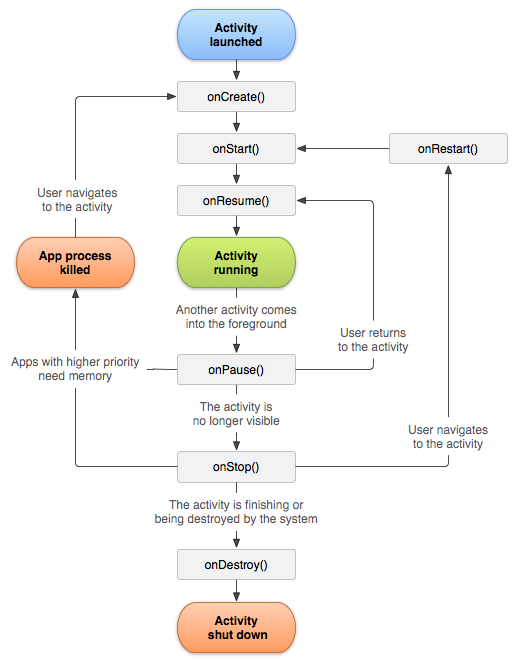
\includegraphics[scale=0.4]{activity_lifecycle}
\caption{Flowchart showing the entire Android Activity lifecycle. May be relevent.}
\label{fig:activity_lifecycle}
\end{figure}

The menu structure of the application is illustrated in figure \ref{fig:menu_structure}. Each of the three screens accessible from the main menu is represented by a subclass of a SessionSetupActivity object and used to initialise the current session. When a session finishes and players exit the Map Display Screen, on return to one of the session setup activities, the onBackPressed() procedure is called resulting in immediately returning to the main menu.

\tikzstyle{activity} = [rectangle, text width=4.5em, text centered, rounded corners, draw]
\tikzstyle{line} = [draw, -latex']
\begin{figure}[ht]
\centering
\begin{tikzpicture}[node distance = 3cm, auto]
	\node [activity] (main) {Main Menu};
	\node [activity, below of=main] (btM) {Bluetooth Device Selection};
	\node [activity, left of=btM] (quickstart) {Quickstart};
	\node [activity, right of=btM] (btC) {Bluetooth Client Screen};
	\node [activity, below of=btM] (map) {Map Display Screen};
	\path [line] (main) -- (quickstart);
	\path [line] (main) -- (btM);
	\path [line] (main) -- (btC);
	\path [line] (quickstart) -- (map);
	\path [line] (btM) -- (map);
	\path [line] (btC) -- (map);
\end{tikzpicture}
\caption{Flowchart showing the possible paths through the activities of the application}
\label{fig:menu_structure}
\end{figure}

The Android Software Development Kit (SDK) offers assistance in creating graphical user interfaces, including a "What you see is what you get" (WYSIWYG) graphical editor. However, for the purposes of this project (simple menu and selection screens) this tool was undesired and in order for the screen arrangements to appear as desired on all screen sizes, it was decided that all GUI work would be done by text entry using relative positioning so no features would be accidentally introduced by the automated tool. Despite this the tool provided value by visualising the changes made to the layout files without having to install it on a device.

\section{Implementing the Session Setup function}

TODO: Whats in a session?

The application structure first implemented left a gap for a session setup module. The reason for this is that there are numerous ways to setup the session and it is conceivable that there may not be an absolute best method.
As further justification, consider the case of using the client server model for main inter-device communications. With this network in place, the server can act as an intermediary when setting up the initial session, since its address is always known by all participants. However, if peer to peer methods alone are used for communication, then there is no oracle that can introduce devices to each other, and some form of ad-hoc discovery method would be required.

For the initial iterations of the app, a trivial single-user module was used to initialise the session, allowing testing of the data storage and visualisation components before further setup modules were implemented. More than just a temporary placeholder, this module allows for users of the complete system to use the system alone if they wish.

The first multi-participant session setup module was designed to be universal, since at the time developing further modules was an optional project extension so this may have been the only one.
This meant that ad-hoc discovery methods would be used since they don't rely on an external provider and can work with both server based and peer to peer systems.

There are several options for such ad-hoc device discovery.

All devices running Android version 2.2 and above that have WiFi are able to host personal WiFi hotspots. One solution to the setup problem would be to have one device set up a hotspot, identify and add all connecting devices to the session, and then distribute the session information back to them over WiFi. For security, Android uses a primitive form of User Account Control (UAC) to ensure that some operations can only be done with explicit user permission, connecting to a new wireless access point is one of these. It is usually desirable for technical implementation detail to be hidden from the user, but this method would violate that guideline and complicate the process unless all users had previously connected to this hosts hotspot.
A similar suggestion is to use Bluetooth as the medium. This would operate in a similar manner, though unlike WiFi connections would be serialised, requiring most devices to connect to the host twice - once to contribute their information, and once to receive the complete session information after it has all been gathered. Androids UAC polilcy only requires user consent for pairing with new bluetooth devices and not for connecting to paired devices. So provided the devices are paired beforehand, the entire process can be automated.
Near Field Communication (NFC) has recently been adopted by handset manufacturers, and allows communication by simply making contact between two NFC enabled devices. QR codes allow communication via a visual channel and could be used by displaying a QR code on one screen while another devices directs their camera towards it. These two methods are similar in that they provide one-to-one communication and require each device to be physically oriented in respect to the other. This means coordinating a large group of devices using these mediums could become a complicated process for the user, even with on screen instruction.

Bluetooth was chosen over WiFi because the connection process is simpler for the user.

Pre-arranged / permanent session - can do with anything anyway

\subsection{Bluetooth Session Setup}
\label{bt setup}
In order to initialise and distribute the session using bluetooth, the following steps are taken:

\begin{itemize}
\item{Master selects bluetooth devices to join from list on screen.}
\item{Meanwhile slave devices select connect and start listening for bluetooth connection.}
\item{Master connects to each selected device in turn, retrieving their address information, as well as any necessary cryptographic information such as private keys.}
\item{Master marshals session object from all of the collected information, including it's own.}
\item{Master connects again to each device in turn and distributes the session object.}
\end{itemize}

\subsection{Remote Server based Session Setup}

While the Bluetooth based method worked well in testing, having to connect to several devices sequentially causes a severe bottleneck in the process.

For this reason, another session setup procedure was built, using a remote server.

To connect, the user of each device presses the same "Quickstart" button. This is the only user activity necessary and is hence more convenient to use.

When the function is activated the location of the device, obtained using a combination of GPS and Network provided data\footnote{See later}, is sent to the server along with the session information of the device.

At the server, these requests are received and grouped by time and location into session groups. From these groups, session objects are marshalled and sent back to the devices involved.

The location information used for grouping is in the form of 2D cartesian coordinates.

\begin{algorithm}
\For{device a: requests}{
 \ForAll{device b: requests} {
  \If{\begin{math}distance(a,b) \leq x \end{math}}{
   a.add(b);
  }
 }
}
\caption{Naive grouping algorithm}
\end{algorithm}

If a naive grouping algorithm was used the run time complexity would be O(n\textsuperscript{2}) where n is the number of devices.
This is avoided by noting that there is an upper limit on the distance between any two devices in the same session. This allows one to segment the 2D location space into a grid of disjoint areas, where comparisons need to be made only between points in adjacent segments. While still technically remaining O(n\textsuperscript{2}) in the worst case (where all devices are close together), in practice there is an upper limit on the number of users that can be in the same place at the same time resulting in an effective O(1) runtime complexity.

In practice when this method is available it is much quicker than the bluetooth based alternative for two reasons. One is the bottle connection bottleneck mentioned in \ref{bt setup} and the other is that it is no longer necessary to select the participants from a list of devices. This comes at the cost of expressiveness since instead all nearby devices are added. An option could be added to allow selection participants without much work.

Clearly the bluetooth method has the advantage of not relying on external providers.

\section{Map Display and Data Structures}

There are several ways the location data could be visualised on screen. The approach taken here is to draw a line to the screen for each user in the session, showing their entire path since the event began. The lines could be super-imposed onto existing map visualisation data such as that provided by Google\footnote{https://developers.google.com/maps/documentation/android/} but with the desire to keep the interface simple and quickly interpretable this wasn't attempted.

\subsection{Storing Location History Data}

For each device, the entire known location history, for the current session, should be stored at every other device so that each device can potentially perform arbitrary computation and aggregation on it.

To do this, a data structure was required that would store a list of (time, location) data points.

The structure chosen was a linked list of array lists. The data-points would be stored in fixed size arrays, where more arrays can be allocated when needed. This means append, lookup and insert have runtime costs of $ O(\lceil N/L \rceil ) $ where $ N = $ number of points and $ L =$ array size.

For each device, this structure is indexed by an integer logical clock governed by the device the data originates from. This allows devices to alter the granularity of history depending on the speed of travel, simply by incrementing its logical clock every time it travels some fixed size distance. It also provides a simple way to check for missing data, since if there exists any empty index i such that i<j where j is the latest known index, then the data for index i is absent and should be seeked out. This is explained further in \ref{requests}.
The alternative would be to index the lists by time, this would suffer from variable path resolution depending on speed, and several undesirable effects such as duplicate locations being stored whenever a device remains stationary.

Since the aim is to fully populate the list with data points up to some logical time l, allocating arrays is not wasteful because any intermediate gaps in the data should be filled in future. The trade off here comes with setting the length of the arrays, too large and more memory will be unused at the end of the array, too small and lookup times will increase because of the increased size of the linked list.

\subsection{Drawing to the Screen}

To present a visualisation to the user, the data points need to be mapped onto a 2D space the size of the devices screen, and lines need to be drawn between them.

The android canvas API provides suitable methods for plotting points, lines and paths to the screen. In this context, a Path object represents an append-only ordered list of points that can be pre-computed and drawn to the screen efficiently at different times.
Being append-only, the Path objects don't provide an immediate solution for drawing entire device paths to the screen for each frame. The reason for this is that at any point in time, there may be absent data points which should be drawn along the path between two present data points. Since these absent points may later be obtained, the data structure should allow for insertion and not just append.

To solve this, a data structure named a PathCache was designed. This is comprised of a Tree Set of Segment objects, where a Segment may be either a Complete Segment or a Gap Segment. Complete segments are parts of the data point list that have no missing data. Gap segments are segments of the list that contain only missing points.

Each Complete segment contains a Path object that can be drawn to the screen.

This structure provides efficient insertion of data points into the lists as well as conserving the efficient append operation when using a single Path object. To append points, they are just appended to the last CompleteSegment (the last segment will never be a GapSegment because gaps are defined as missing data points with index less than that of the largest index received.). To insert points there are two possible cases. Either the new point is at the start of a GapSegment, in which case it is appended to the preceeding CompleteSegment, and the GapSegment is shortened by one. If the new point is not at the start of a GapSegment (meaning it is somewhere else in some GapSegment) then the GapSegment is shortened, a single point CompleteSegment added, and if the point wasn't at the end of the GapSegment, then an extra GapSegment is added to fill in the rest of the old GapSegment. The TreeSet provides mapping from indices to Segments (as well as preceding Segments) in O(log(N)) time.

To draw the paths to the screen each frame, every segment is iterated through and drawn, with individual lines being drawn between them to replace the gap segments.

+player labels and naming?

When scanning through the Path objects, the boundaries are calculated, these are the maximum and minimum coordinates on each axis. These are used to calculate the scale factor required to map the life-size model to the scale of the screen. A matrix is constructed from this factor and applied to transform each of the paths, and they are shifted to be aligned at (0,0).

\section{Data Sharing}

As mentioned earlier the networking parts of the system were sufficiently loosely coupled to enable modular swapping of different protocols. This was achieved using standard OOP conventions and the use of an abstract class ProtocolManager which was subclassed by the various different networking implementations.

The approach taken was initially a simple bucket and send protocol. This means that as new points arrive from the location aware part of the system, they are put into a bucket and sending is delayed until either the bucket is full or the first item in the bucket has been there more than some fixed amount of time.

This prevents excessive sending delay while not abusing the network by sending many smaller than necessary packets, as was seen to be a problem in \ref{3g queue delay}.





\cleardoublepage
\chapter{Evaluation}

To do.

Include:
\begin{itemize}
\item{Differing characteristics of UK phone networks (Vodafone and Three)}
\end{itemize}

\cleardoublepage
\chapter{Conclusion}

To do.

\cleardoublepage

%%%%%%%%%%%%%%%%%%%%%%%%%%%%%%%%%%%%%%%%%%%%%%%%%%%%%%%%%%%%%%%%%%%%%
% the bibliography

\addcontentsline{toc}{chapter}{Bibliography}
\bibliography{refs}
\cleardoublepage

%%%%%%%%%%%%%%%%%%%%%%%%%%%%%%%%%%%%%%%%%%%%%%%%%%%%%%%%%%%%%%%%%%%%%
% the appendices
\appendix

\chapter{Project Proposal}

%
% Draft #1 (final?)

\vfil

\centerline{\Large Computer Science Project Proposal}
\vspace{0.4in}
\centerline{\Large How to write a dissertation in \LaTeX\ }
\vspace{0.4in}
\centerline{\large M. Richards, St John's College}
\vspace{0.3in}
\centerline{\large Originator: Dr M. Richards}
\vspace{0.3in}
\centerline{\large 14$^{th}$ October 2011}

\vfil


\noindent
{\bf Project Supervisor:} Dr M. Richards
\vspace{0.2in}

\noindent
{\bf Director of Studies:} Dr M. Richards
\vspace{0.2in}
\noindent
 
\noindent
{\bf Project Overseers:} Dr~F.~H.~King  \& Dr~A.~W.~Moore


% Main document

\section*{Introduction, The Problem To Be Addressed}


Many students write their CST dissertations in \LaTeX\ and
spend a fair amount of time learning just how to do that. The purpose of 
this project is to write a demonstration dissertation that explains in
detail how it done.  

This core proposal document will be augmented by a separately-printed
cover sheet at the front and a resource form at the end.  Additional
sheets for risk assessment and human resources may also need to be included.

This document will repeat much of the material that is summarised on the additional sheets.

\section*{Starting Point}

{\em Describe existing state of the art, previous work in this area, libraries and databases to be used.
Describe the state of any existing codebase that is to be built on.  }

I am already able to write prose using the English language. I have an online dictionary. etc..

\section*{Resources Required}

{\em A note of the resources required and confirmation of access.}

For this project I shall mainly use my own quad-core computer that runs Fedora Linux. Backup
will be to github and/or to an SVN repository on an external hard disk that is dumped to writable CD/DVD media.
I have another similar computer to hand should my main machine suddenly fail.
I require no other special resources.

\section*{Work to be done}

{\em Describe the technical work.}

The project breaks down into the following sub-projects:

\begin{enumerate}

\item The construction of a skeleton dissertation with the required 
structure. This involves writing the Makefile and makeing dummy files
for the title page, the proforma, chapters 1 to 5, the appendices and
the proposal.

\item Filling in the details required in the cover page and proforma.

\item Writing the contents of chapters 1 to 5, including examples
of common \LaTeX\ constructs.

\item Adding a example of how to use floating figures and encapsulated
postscript diagrams.

\end{enumerate}

\section*{Success Criterion for the Main Result}


The project will be a success if I have a completed dissertation with the correct chapter
titles and I have achieved my other success criterion, which is to blah ...



\section*{Possible Extensions}

{\em Potential further envisaged evaluation metrics or extensions.}

If I achieve my main result early I shall try the following alternative experiment or method of evaluation ...


\section*{Timetable: Workplan and Milestones to be achieved.}


{\em Perhaps list ten or so  two-week work-packages.}

Planned starting date is 16/10/2011.

\begin{enumerate}

\item {\bf Michaelmas weeks 2-4} Learn to use X. Read book Y. Read papers Z.

\item {\bf Michaelmas weeks 5-6} Do preliminary test of Q.

\item {\bf Michaelmas weeks 7-8} Start implementation of main task A.

\item {\bf Michaelmas vacation} Finish A and start main task B.

\item {\bf Lent weeks 0-2} Write progress report. Generate corpus of test examples. Finish task B.  

\item {\bf Lent weeks 3-5} Run main experiments and achieve working project.

\item {\bf Lent weeks 6-8} Second main deliverable here.

\item {\bf Easter vacation:} Extensions and writing dissertation main chapters.

\item {\bf Easter term 0-2:}  Further evaluation and complete dissertation.

\item {\bf Easter term 3:} Proof reading and then an early submission so as to concentrate on examination revision.

\end{enumerate}


 



\end{document}
